% fig-primitives — §3, the four primitives (DID -> VC -> IPR -> Trust Score).
% Standalone-buildable AND \input-able. Uniform boxes, muted palette (figures/colors.tex),
% Trust Score = accent (the aggregating element).
\documentclass[border=4pt]{standalone}
\usepackage{tikz}
\usetikzlibrary{positioning,arrows.meta}
% figures/colors.tex — shared, muted, arXiv-safe palette for all four figures.
% Change colours HERE; all four figures + the paper pick it up.
% Requires xcolor (loaded by tikz / the paper). \input-able in a preamble.
\definecolor{figline}{HTML}{3A4A5A}        % muted slate-blue — outlines + text (standard)
\definecolor{figfill}{HTML}{ECF1F6}        % very light blue-grey — standard node fill
\definecolor{figaccent}{HTML}{2E6E66}      % muted teal — central / key element outline
\definecolor{figaccentfill}{HTML}{DBEAE6}  % light teal — central element fill
\definecolor{figmuted}{HTML}{6B7785}       % muted grey — labels / secondary text

\begin{document}
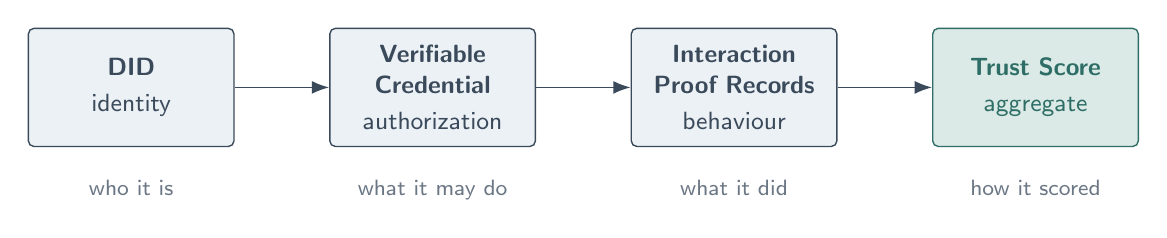
\begin{tikzpicture}[
  node distance=12mm,
  pbox/.style={draw=figline, line width=0.5pt, rounded corners=2pt, align=center,
               text=figline, font=\small\sffamily, fill=figfill,
               text width=24mm, minimum height=15mm, inner sep=3pt},
  pacc/.style={pbox, draw=figaccent, fill=figaccentfill, text=figaccent},
  flow/.style={-{Latex[length=2.2mm]}, draw=figline, line width=0.6pt},
  clab/.style={font=\footnotesize\sffamily, text=figmuted}
]
\node[pbox] (did) {\textbf{DID}\\[2pt]identity};
\node[pbox, right=of did] (vc)  {\textbf{Verifiable Credential}\\[2pt]authorization};
\node[pbox, right=of vc]  (ipr) {\textbf{Interaction Proof Records}\\[2pt]behaviour};
\node[pacc, right=of ipr] (ts)  {\textbf{Trust Score}\\[2pt]aggregate};
\draw[flow] (did) -- (vc);
\draw[flow] (vc)  -- (ipr);
\draw[flow] (ipr) -- (ts);
\node[clab, below=3mm of did] {who it is};
\node[clab, below=3mm of vc]  {what it may do};
\node[clab, below=3mm of ipr] {what it did};
\node[clab, below=3mm of ts]  {how it scored};
\end{tikzpicture}
\end{document}
